\chapter{Annotations}
\label{chap:annotations}

Annotations allow a study to collect custom named and defined pieces of data
for participants, collection events, and specimen processing. Figure
\ref{fig:annotation-example} shows the annotation entities related to
participant annotations. The annotations for collection event and specimen
processing are similar. Annotations are optional and are not required to be
defined for a study.

\begin{figure}[H]
  \centering
  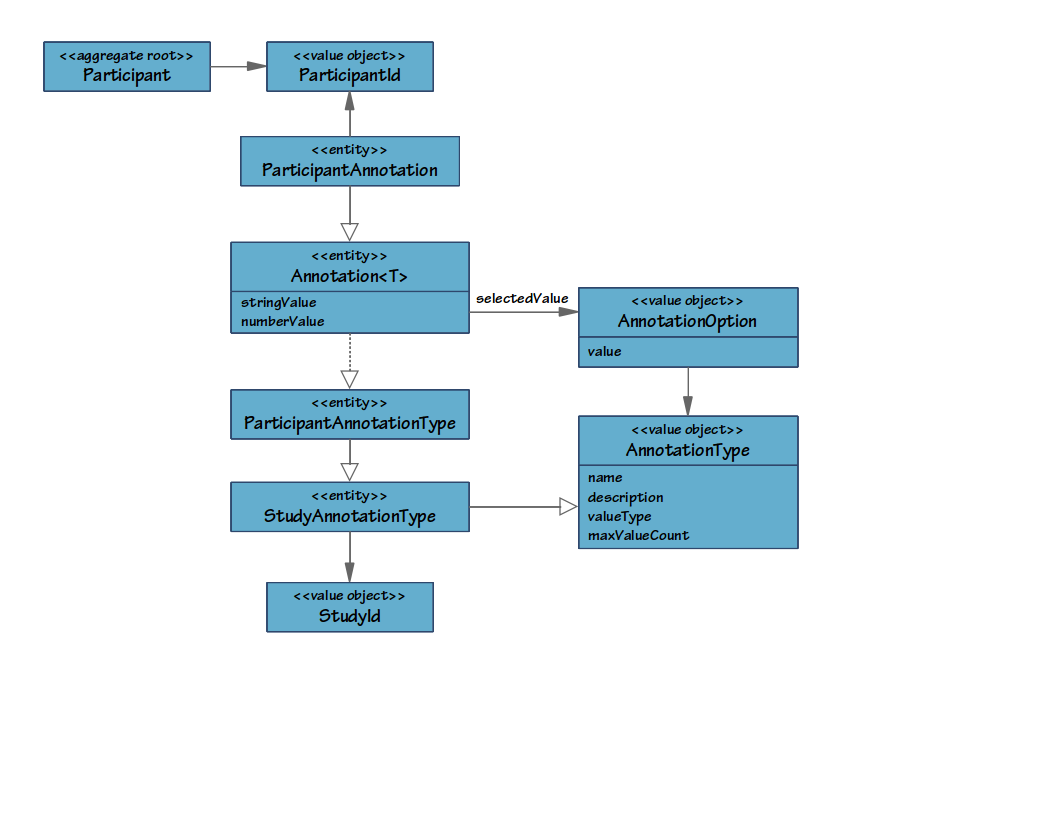
\includegraphics[trim={10mm 45mm 68mm 10mm}, clip,
    width=0.8\textwidth]{images/annotation-example}
  \caption{Annotations example}
  \label{fig:annotation-example}
\end{figure}

The \entitylink{ParticipantAnnotation} is a derived class of the generic class
\entitytarget{Annotation}. Possible annotations for a study are defined using
\entitylink{ParticipantAnnotationType} which is a derived class for
\entitylink{StudyAnnotationType} which itself is a derived class of
\entitytarget{AnnotationType}.

An annotation type has a short identifying name that is unique to the study. A
description can also be defined but is optional. The following table shows the
possible values for \compfont{valueType}. The value type specifies what the
annotation stores.

\begin{table}[H]
\renewcommand{\arraystretch}{1.1}
\begin{tabularx}{\textwidth}{@{\hspace{6pt}} >{\ttfamily}l X }
  \sffamily{\textbf{Value Type}} & \sffamily{\textbf{What is stored}}\\
  \hline

  String & an alphanumeric string.\\
  Number & a number, either integer or decimal.\\
  Date & date string, usually of the form \emph{YYYY-MM-DD HH:MM}.\\
  Select & a value selected from a predefined list.\\

\end{tabularx}
\end{table}

When \compfont{valueType} is assigned to be of type \compfont{Select},
\compfont{maxValueCount} is the number of of items that can be selected from the
predefined list. If only one value is allowed, then \compfont{maxValueCount} has
a value of 1. If an unlimited number of values are allowed then,
\compfont{maxValueCount} has a value of 0.

One or more \entitylink{AnnotationOption}s are used to create the predefined
list of select options.

Of the fields \compfont{stringValue}, \compfont{numberValue}, or
\compfont{selectedValue} in \entitytarget{Annotation}, only a single one is
used to store the annotation value. The remaining fields are
\compfont{null}. The field that is used is referred to as the \emph{Value
  Field}. The Value Field used depends on the value
\compfont{AnnotationType.valueType}.

\begin{table}[!htbp]
\renewcommand{\arraystretch}{1.1}
\begin{tabularx}{\textwidth}{@{\hspace{6pt}} >{\ttfamily}l l}
  \sffamily{\textbf{ValueType}} & \sffamily{\textbf{Value field}}\\
  \hline
  String & \compfont{stringValue}\\
  Number & \compfont{numberValue}\\
  Date & \compfont{numberValue} and stored as the number of seconds\\
  Select & \compfont{selectedValue}\\

\end{tabularx}
\end{table}
